%!TEX program = xelatex
% 完整编译: xelatex -> biber/bibtex -> xelatex -> xelatex
\documentclass[lang=cn,11pt,a4paper]{elegantpaper}

\title{height.h说明文档}
\author{Haochen Huang}

\version{1.02}
\date{\zhtoday}



% 本文档命令
\usepackage{array}

\begin{document}

\maketitle
\begin{abstract}
    本文档为height.h说明文档的测试初稿版本,需要继续的工作包括对树状网格函数部署的相关代码解析,整体算法的高度总结,对代码中各种数值加密的详细解析等\par
    1.02更新,根据反馈更改了大量注释,对图例进行了阐释
\end{abstract}

\tableofcontents

\section{height.h整体头文件目的}
本头文件是构造多相流边界几何的必要工具头文件之一,其与parabola.h共同为curvature.h服务,计算实现边界面的曲率。相关算法的具体细节请参考\cite{popinet2009accurate}

\section{heights函数整体循环框架与具体实现}
\subsection{height整体循环框架}
由于height.h文件框架相当特殊,两个主要函数相互耦合才能完全展示整个循环,是故不分别撰写half column与heights函数。\par
heights函数的目的是遍历该单元所有方向(二维2个方向,三维3个方向)上的正负4个单元,并求出该单元的高度函数值,存储在vector型数据中。两函数在此过程中的作用分别是:
\begin{enumerate}
    \item half column函数通过传递的参数,求解所有维度上单一方向的height函数值,并在heights函数对方向进行循环时更新完整的height函数值并返回。
    \item heights函数通过调用half column并通过对参数$j$的循环达到正负方向的遍历。
\end{enumerate}
由于各个方向的高度相似性,下文中我们均以二维问题中x方向的情况作为例子。\par
接下来我们对高度函数值进行解析定义。\par
一个单元的高度函数值得重要条件是空间上的循环\textbf{完整}地通过一个界面,即在界面前后都找到$c=0,c=1$的单元格,如下图情况所示(本文中图例仅作参考,实际运用过程中会有所不同,请读者按照代码仔细甄别,在curvature.h中会具体分析)
\begin{figure}[H]
    \begin{center}
    \subfigure[a]{
    \begin{minipage}[t]{0.58\linewidth}
    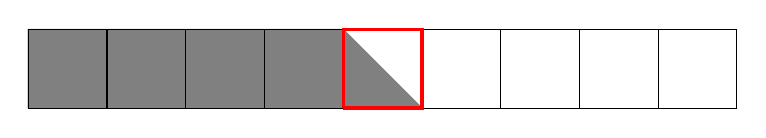
\begin{tikzpicture}[scale=1]
        \filldraw[gray] (-4.0,0)--(1.0,0)--(0,1)--(-4.0,1)--(-4.0,0);
        \draw[step=1cm] (-4.0,0) grid (5.0,1.0);
        \draw[very thick,red] (0,0)--(0,1)--(1,1)--(1,0)--(0,0);
    \end{tikzpicture}
    \end{minipage}
    }
    
    
    \subfigure[b]{
    \begin{minipage}[t]{0.58\linewidth}
    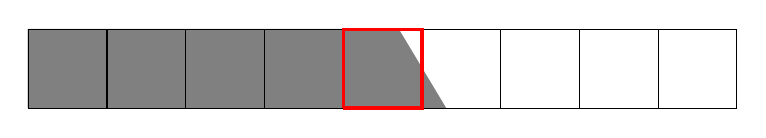
\begin{tikzpicture}[scale=1]
        \filldraw[gray] (-4.0,0)--(1.3,0)--(1.0,0.5)--(0.7,1)--(-4.0,1)--(-4.0,0);
        \draw[step=1cm] (-4.0,0) grid (5.0,1.0);
        \draw[very thick,red] (0,0)--(0,1)--(1,1)--(1,0)--(0,0);
    \end{tikzpicture}
    \end{minipage}
    }
    
    \subfigure[c]{
    \begin{minipage}[t]{0.58\linewidth}
    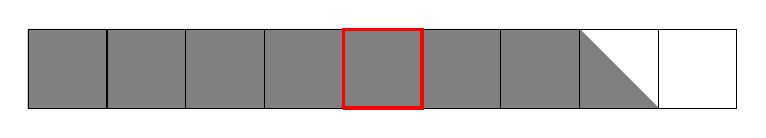
\begin{tikzpicture}[scale=1]
        \filldraw[gray] (-4.0,0)--(4.0,0)--(3.0,1)--(-4.0,1)--(-4.0,0);
        \draw[step=1cm] (-4.0,0) grid (5.0,1.0);
        \draw[very thick,red] (0,0)--(0,1)--(1,1)--(1,0)--(0,0);
    \end{tikzpicture}
    \end{minipage}
    }
    \end{center}
    \caption{高度函数值可定义情况示例}
\end{figure}
其中灰色部分代表界面内部,白色代表界面外侧,红色方框代表当前单元。在这种情况下高度函数有定义。\par
如不满足上述条件的网格情况,高度函数在该单元上没有定义,算法会对单元赋值$nodata$(一个极大的数值,在common.h中定义),如下图\ref{fig:bukedingyi}
\begin{figure}[H]
\centering

    \subfigure[d]{
    \begin{minipage}[t]{0.58\linewidth}
    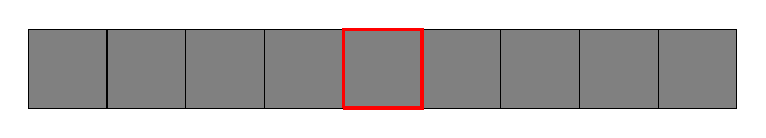
\begin{tikzpicture}[scale=1]
        \filldraw[gray] (-4.0,0)--(5.0,0)--(5.0,1)--(-4.0,1)--(-4.0,0);
        \draw[step=1cm] (-4.0,0) grid (5.0,1.0);
        \draw[very thick,red] (0,0)--(0,1)--(1,1)--(1,0)--(0,0);
    \end{tikzpicture}
    \end{minipage}
    }
   
    \subfigure[e]{
    \begin{minipage}[t]{0.58\linewidth}
    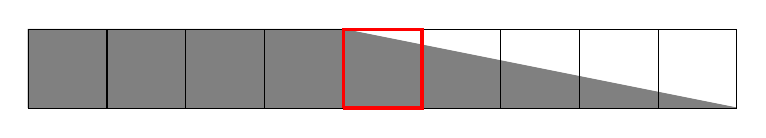
\begin{tikzpicture}[scale=1]
        \filldraw[gray] (-4.0,0)--(5,0)--(0.0,1)--(-4.0,1)--(-4.0,0);
        \draw[step=1cm] (-4.0,0) grid (5.0,1.0);
        \draw[very thick,red] (0,0)--(0,1)--(1,1)--(1,0)--(0,0);
    \end{tikzpicture}
    \end{minipage}
    }

    \subfigure[f]{
    \begin{minipage}[t]{0.58\linewidth}
    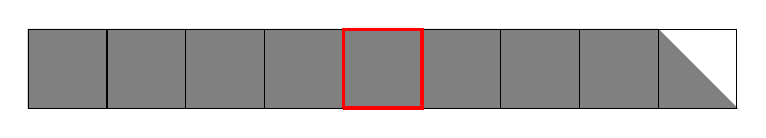
\begin{tikzpicture}[scale=1]
        \filldraw[gray] (-4.0,0)--(5.0,0)--(4.0,1)--(-4.0,1)--(-4.0,0);
        \draw[step=1cm] (-4.0,0) grid (5.0,1.0);
        \draw[very thick,red] (0,0)--(0,1)--(1,1)--(1,0)--(0,0);
    \end{tikzpicture}
    \end{minipage}
    }
    \caption{高度函数不可定义情况示例}\label{fig:bukedingyi}
\end{figure}
高度函数的本质是单元界面内体积分数的加和,各个单元表示量以单元中心线为基准,零标准面处于\textbf{界面开始与界面终结阶段的数值点},如图:
\begin{figure}[H]
    \centering
     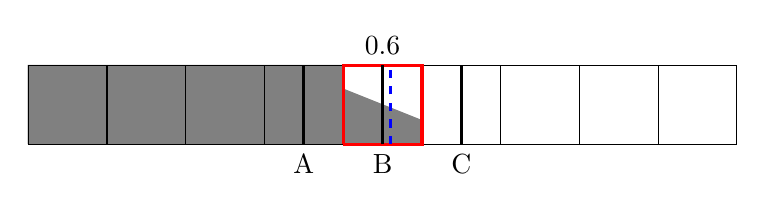
\begin{tikzpicture}[scale=1]
        \filldraw[gray] (-4.0,0)--(1.0,0)--(1.0,0.3)--(0.0,0.7)--(0.0,1)--(-4.0,1)--(-4.0,0);
        \draw[step=1cm] (-4.0,0) grid (5.0,1.0);
        \draw[very thick,red] (0,0)--(0,1)--(1,1)--(1,0)--(0,0);
        \node at (0.5,1.25) {0.6};
        \draw[very thick,dashed,blue] (0.6,0)--(0.6,1);
        \draw[very thick](0.5,0)--(0.5,1);
        \draw[very thick](-0.5,0)--(-0.5,1);
        \draw[very thick](1.5,0)--(1.5,1);
        \node at (-0.5,-0.25) {A};
        \node at (0.5,-0.25) {B};
        \node at (1.5,-0.25) {C};
    \end{tikzpicture}
    \caption{高度函数值示例图}
\end{figure}
图中界面部分体积分数为$0.6$,ABC三个单元即为“界面的开始与界面的终结”故其零标准面在距离A左端1.6长度处($1+0.6$)为图中蓝色点划线,而各个单元中存储的数据为位于单元中心的黑色直线代表的函数高度,计算方法为从零界面开始,坐标正方向递减,负方向增加。ABC所储存的函数值分别为$1.1,0.1,-0.9$。\par
规定由界面内部指向界面外为一个界面的方向(由$1\geq c>0$指向$c=0$),得到的相关结果如图\ref{fig:shuzhishili}\par
图中E处为界面位置,可以看到该函数利用数值非常巧妙的表达了界面方向,即当坐标正方向与界面方向一致时,高度函数值为$(-5,5)$,当相互反向时,高度函数值为$(15,25)$。\par
\begin{figure}[H]
    \centering
        \begin{tikzpicture}
        \draw[step=1cm] (-4.0,0) grid (5.0,1.0);
        \draw (0,1)--(1,0);
        \node at (-0.5,0.5) {B};
        \node at (-1.5,0.5) {A};
        \node at (0.5, 1.5) {E};
        \node at (1.5, 0.5) {C};
        \node at (2.5, 0.5) {D};
        \draw[->] (0,-0.5)--(-3,-0.5) node[anchor=east]{方向1};
        \draw[->] (1,-0.5)--(4,-0.5) node[anchor=west]{方向2};
        \end{tikzpicture}
        \caption{具体数值结果示例}\label{fig:shuzhishili}
\end{figure}
\begin{table}[H]
    \centering
    \begin{tabular}{|c|c|c|c|c|c|}
    \hline
        方向$\backslash$位置序号 & A & B & E & C & D \\ \hline
        方向1 & 22 & 21 & 20 & 19 & 18 \\ \hline
        方向2 & 2 & 1 & 0 & -1 & -2 \\ \hline
    \end{tabular}
    \caption{不同界面方向下各个位置的高度函数值,为了简化流程,界面为平分单元界面}
\end{table}
接下来介绍在代码实现中的算法。\par
\begin{algorithm}[H]
    \caption{Height主题循环框架}
	\label{alg:循环}
	\KwIn{全场各个单元的体积分数$c$,总维度DIMENSION}
	\KwOut{全场各个单元的高度函数值$h$,vector型数据}
	\BlankLine
	\For{$dimension = 1;dimension<=DIMENSION;dimension++$}{
	    设定当前维度的高度函数值h.dimension[];\\
	    \For{$j = -1;j<=1;j+=2$}
	    {
	        \For{$i = 0;i<=4;i++$}
	        {
	            $h.dimension[]+=c[i\times j]$;\\
	            \If{$(c[]==0\&\&c[i\times j]==1)||(c[]==1\&\&c[i \times j]==1)$}
	            {这代表此时循环已经完全穿透整个界面,根据相关方程计算当前单元的高度函数值}
	            \If{$0<c[]<1$}
	            {代表本身处于边界上,需要双方向循环计算积累,判断该单元的函数值}
	            \If{并未发现边界或在循环过程中没有穿透边界}{需要双方向循环判断是否能后返回高度函数值}
	        }
	    }
	}
	return $h$;\\
\end{algorithm}
更多的实现细节需要完整的推演以及仔细阅读相应的代码注释,语言文字并不能完整的描述整个精妙的循环过程,读者在阅读推演代码时需要注意几个问题:
\begin{enumerate}
    \item HSHIFT的使用方式:代码定义HSHIFT为全环境静态值20,目的是区分界面方向,代码中使用该数值对高度函数值进行加密
    \item 多次循环的数据清零问题:在具体代码中方向控制参数与真正计算高度函数的half column是相互分离的,在每次方向循环时,half column中自定义的S H会被清零
    \item 数据的格式以及100加密:函数在表达当前的找寻状态时启用并定义了参数S,它在第二次正向循环时会被int型数据s赋值;由于s会忽视小数,这给了代码使用100对数据进行加密再解析的条件
\end{enumerate}


\subsection{heights及half column源代码及注释}
\begin{minted}[mathescape=true,breaklines]{lexer.py:DiffLexer -x}
/**
# Height-Functions

The "height-function" is a vector field which gives the distance,
along each coordinate axis, from the center of the cell to the closest
interface defined by a volume fraction field. This distance is
estimated using the "column integral" of the volume fraction in the
corresponding direction. This integral is not always defined (for
example because the interface is too far i.e. farther than 5.5 cells
in our implementation) in which case the value of the field is set to
*nodata*. See e.g. [Popinet, 2009](references.bib#popinet2009) for
more details on height functions.

We also store the "orientation" of the height function together with
its value by adding *HSHIFT* if the volume fraction is unity on the
"top" end. The function below applied to the value will return the
corresponding height and orientation.

The distance is normalised with the cell size so that the coordinates
of the interface are given by

~~~c
(x, y + Delta*height(h.y[])) or (x + Delta*height(h.x[]), y)
~~~
*/

#define HSHIFT 20.//区分正方向

static inline double height (double H) {//内联函数,通过文本替换的方式减少函数内存的调用
  return H > HSHIFT/2. ? H - HSHIFT : H < -HSHIFT/2. ? H + HSHIFT : H;//先行判断H是否大于HSHIFT/2.再以此类推
}//本函数的作用是规范高度值,将其完美限定在[-10,10]之间

static inline int orientation (double H) {
  return fabs(H) > HSHIFT/2.;
}

/**
We make sure that two layers of ghost cells are defined on the
boundaries (the default is one layer). */

#define BGHOSTS 2

/**
## Half-column integration 

This helper function performs the integration on half a column, either
"downward" (*j = -1*) or "upward" (*j = 1*). */
//计算从本网格往一个方向延伸4个网格范围内的高度函数值,初始界面网格中高度函数参考值为20,延伸两侧分别递增和递减,本函数为一个工具函数

static void half_column (Point point, scalar c, vector h, vector cs, int j)//h是指针,需要填充操作
{

  /**
  The 'state' of the height function can be: *complete* if both
  ends were found, zero or one if one end was found and between zero
  and one if only the interface was found. */

  const int complete = -1;

  foreach_dimension() {//注意其计算了各个方向的高度函数

    /**
     *S* is the state and *H* the (partial) value of the height
     function. If we are on the (first) downward integration (*j =
     -1*) we initialise *S* and *H* with the volume fraction in
     the current cell. */

    double S = c[], H = S, ci, a;
    //需要提醒的是在每一次j的数值变化后,S,H将会被归零
    /**
     On the upward integration (*j = 1*), we recover the state of the
     downward integration. Both the state and the (possibly partial)
     height value are encoded in a single number using a base 100
     shift for the state. */
    
    typedef struct { int s; double h; } HState;
    HState state = {0, 0};
    if (j == 1) {//在调用本函数时,j的初始值被设定为-1,所以阅读时请从-1看起
    /*在第二次循环(j==1)时会进入本判断语句,本段代码的主要作用就是设置表示当前循环状态的S值。
    当上一个循环完整通过界面后,h.x[]会被赋值为小于25的数值(这取决于其方向),是故在接下来的判断操作中,int s会取为0,S则被设定为-1,代表已经完成循环。
    当上一个循环没有找到界面或没有通过界面一端;
    即向负方向循环遍历后并没有
    1.初始位置$1\geq c>0$,然而在负方向循环上没有出现$c[]=1$或$c[]=0$
    2.初始位置$c[]=1$或$c[]=0$在负方向循环上没有出现$c[]=0$或$c=1$
    S会保持为c[]向另一个方向进行遍历,以求得通过界面获得定义,而在此之前state.s会被提前设置为-1,state,h会被提前设置为nodata。
    而当初始单元处于界面上即$1\geq c>0$在负方向循环中找到单元$c[]=1$或$c[]=0$此时S则会被赋值为1或0,表示已经完整一半,并记录方向*/
      /**
      Check whether this is an inconsistent height. */

      if (h.x[] == 300.)//inconsistent
	        state.s = complete, state.h = nodata;//nodata就意味着没有找到边界,或者无法定义

      /**
      Otherwise, this is either a complete or a partial height. */
      
      else {
            int s = (h.x[] + HSHIFT/2.)/100.;//注意这里是int值,小数归零
            state.h = h.x[] - 100.*s;
            state.s = s - 1;
      }

      /**
      If this is a complete height, we start a fresh upward
      integration. */
      
      if (state.s != complete)
            S = state.s, H = state.h;
    }
    
    /**
     We consider the four neighboring cells of the half column, the
     corresponding volume fraction *ci* is recovered either from the
     standard volume fraction field *c* (first two cells) or from the
     shifted field *cs* (last two cells). The construction of *cs* is
     explained in the next section. */
    
    for (int i = 1; i <= 4; i++) {//即开始对某一个方向上的单元进行循环,依次判定是否经过包含边界的单元,以及是否是填充/全空单元
      ci = i <= 2 ? c[i*j] : cs.x[(i - 2)*j];//cs即为下文heights函数中的s,cs[]为c[2*j]即向j方向移动两单元格后的体积分数值
      H += ci;//对高度函数进行累加
      
      /**
       We then check whether the partial height is complete or not. */
      
      if (S > 0. && S < 1.) {//即此时起始单元所处位置恰好在边界上
            S = ci;
            if (ci <= 0. || ci >= 1.) {//若不能进入该循环,说明下一循环单元还是包含界面
      
      /**
       We just left an interfacial cell (*S*) and found a full or
       empty cell (*ci*): this is a partial height and we can stop
       the integration. If the cell is full (*ci = 1*) we shift
       the origin of the height. */
    
                H -= i*ci;//将初始坐标定在界面内距离界面一格的地方
                break;
            }
    }
      
      /**
       If *S* is empty or full and *ci* is full or empty, we went
       right through he interface i.e. the height is complete and
       we can stop the integration. The origin is shifted
       appropriately and the orientation is encoded using the "HSHIFT
       trick". */
      
      else if (S >= 1. && ci <= 0.) {//下两种用于判断起始单元位置在界面内/外,循环单元已变为完全界面外/内单元
            H = (H - 0.5)*j + (j == -1)*HSHIFT;//HSHIFT就是用来辨别处理方向的,当该判别启动时最终的H数值会增长畸变大于10
            S = complete;
            break;
      }
      else if (S <= 0. && ci >= 1.) {//此二者全部将状态设置为complete原因是成功通过了边界
            H = (i + 0.5 - H)*j + (j == 1)*HSHIFT;
            S = complete;
            break;
      }
      
      /**
       If *ci* is identical to *S* (which is empty or full), we
       check that *H* is an integer (i.e. its fractional value is
       zero), otherwise we are in the case where we found an
       interface but didn't go through it: this is an
       inconsistent height and we stop the integration. */
      
      else if (S == ci && modf(H, &a))//modf()的功能是提取double的整数与小数部分,因为如果经过的单元都是界面内或外,其H必定为整数,modf()必定为0,否则就是并没有完全穿透一个界面
            break;
    }

    /**
     We update the global state using the state *S* of the
     half-integration. */
    
    if (j == -1) {

      /**
       For the downward integration, we check that the partial heights
       (*S != complete*) are consistent: if the first cell is full
       or empty or if the last cell is interfacial, the partial
       height is marked as inconsistent. */
      
      if (S != complete && ((c[] <= 0. || c[] >= 1.) ||
            (S > 0. && S < 1.)))
            /*当当前状态并非完成且(原始单元并非全满/全空或最终单元在界面上),根据上一循环,进入该判断条件的应该为
            1.单元负方向循环过程中找到界面,但最终没有完整通过界面
            2.在整个循环中单元全部保持$c[]=1$或$c[]=0$*/
            h.x[] = 300.; // inconsistent,一旦被赋此值,直接会认定为nodata
      else if (S == complete)
            h.x[] = H;
      else//根据上一循环,有一种情况会进入该判断1.起始单元位于边界面上,循环单元完全离开边界面,此时S被赋值为循环单元值

    /**
    This is a partial height: we encode the state using a base 100
    shift. */
    
            h.x[] = H + 100.*(1. + (S >= 1.));//100加密操作,用于判断在该情况下S>=1是否成立,用于判断界面外向方向,若S>=1则说明其脱离界面进入界面内,界面方向与正方向相同,若不成立,则说明界面方向与正方向相反
    }
    else { // j = 1

      /**
       For the upward integration, we update the current *state*
       using the state of the half-integration *S* only if the
       first downward integration returned a partial height, or if
       the upward integration returned a complete height with a
       smaller value than the (complete) height of the downward
       integration. */
      
      if (state.s != complete ||
      (S == complete && fabs(height(H)) < fabs(height(state.h))))//对于之前没有完成的情况,进行数据更新,其中第二个满足条件为在向负方向循环并没有找到界面,正方向循环后寻找到完整的界面
            state.s = S, state.h = H;
      
      /**
       Finally, we set the vector field *h* using the state and
       height. */
      
      if (state.s != complete)//即在正负方向上都没有找到两个端点
            h.x[] = nodata;
      else
            h.x[] = (state.h > 1e10 ? nodata : state.h);
    }
  }
}

/**
## Multigrid implementation

The *heights()* function takes a volume fraction field *c* and returns
the height function vector field *h*. */
//计算网格4个网格范围内各个方向的高度函数

#if !TREE
trace
void heights (scalar c, vector h)
{

  /**
  We need a 9-points-high stencil (rather than the default
  5-points). To do this we store in *s* the volume fraction field *c*
  shifted by 2 grid points in the respective directions. We make sure
  that this field uses the same boundary conditions as *c*. */
  
  vector s[];
  foreach_dimension()
    for (int i = 0; i < nboundary; i++)
      s.x.boundary[i] = c.boundary[i];

  /**
  To compute the height function, we sum the volume fractions in a
  (half-)column starting at the current cell. We start by integrating
  downward (*j = -1*) and then integrate upward (*j = 1*). */
  
  for (int j = -1; j <= 1; j += 2) {

    /**
    We first build the shifted (by $\pm 2$) volume fraction field in each
    direction. */
    
    foreach()
      foreach_dimension()
        s.x[] = c[2*j];

    /**
    We sum the half-column, downward or upward. We (exceptionally)
    need to allow for stencil overflow. */

    foreach (overflow)
      half_column (point, c, h, s, j);
  }

  /**
  Finally we "propagate" values along columns. */
  
  column_propagation (h);
}
\end{minted}
\section{column propagation函数}
\subsection{函数目的及原理}
本函数的目的为:对靠近边界(5.5个单元长度内)但由于算法被赋值nodata的单元进行高度函数赋值。\par
如下图:
\begin{figure}[H]
    \centering
     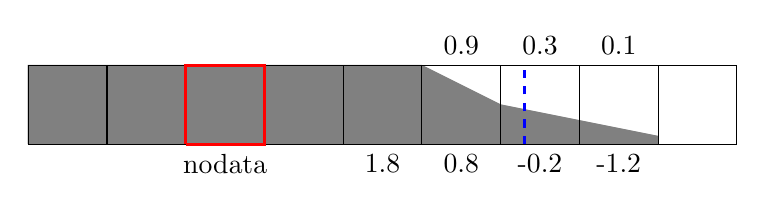
\begin{tikzpicture}[scale=1]
        \filldraw[gray] (-4.0,0)--(4.0,0)--(4.0,0.1)--(3.0,0.3)--(2.0,0.5)--(1.0,1)--(-4.0,1)--(-4,0);
        \draw[step=1cm] (-4.0,0) grid (5.0,1.0);
        \draw[very thick,red] (-2,0)--(-2,1)--(-1,1)--(-1,0)--(-2,0);
        \node at (1.5,1.25) {0.9};
        \node at (2.5,1.25) {0.3};
        \node at (3.5,1.25) {0.1};
        \draw[very thick,dashed,blue] (2.3,0)--(2.3,1);
        \node at (0.5,-0.25) {1.8};
        \node at (1.5,-0.25) {0.8};
        \node at (2.5,-0.25) {-0.2};
        \node at (3.5,-0.25) {-1.2};
        \node at (-1.5,-0.25) {nodata};
    \end{tikzpicture}
    \caption{column propagation函数值示例图}
\end{figure}
图中红色方框中的单元正负方向9个单元长度内都没有完整的通过边界,是故在half column中,其高度函数h被赋值为nodata,经过column propagation之后被赋值为3.8。
\subsection{column propagation函数源代码及注释}
\begin{minted}[mathescape=true,breaklines]{lexer.py:DiffLexer -x}
/**
## Column propagation

Once columns are computed on a local 9-cells-high stencil, we will
need to "propagate" these values upward or downward so that they are
accessible at distances of up to 5.5 cells from the interface. This is
important in 3D in particular where marginal (~45 degrees) cases may
require such high stencils to compute consistent HF curvatures. We do
this by selecting the smallest height in a 5-cells neighborhood along
each direction. */

static void column_propagation (vector h)
{
  foreach (serial) // not compatible with OpenMP
    for (int i = -2; i <= 2; i++)
      foreach_dimension()
          if (fabs(height(h.x[i])) <= 3.5 &&
          fabs(height(h.x[i]) + i) < fabs(height(h.x[])))//该函数目的是保证远端靠近界面的nodata型被赋值
            h.x[] = h.x[i] + i;
}
\end{minted}
\printbibliography[heading=bibintoc, title=\ebibname]
\end{document}
